% ==============================================================================
% 
% Copyright or (c) or Copr. the PyPHS Organization,
% team S3AM, IRCAM Laboratory, CNRS - UMR 9912 STMS,
% 1 place Igor Stravinsky, F-75004 Paris
% * contributors : Antoine Falaize, Thomas Helie,
% * corresponding contributor: antoine.falaize@ircam.fr
% 
% This file has been generated by the Python software PyPHS, which purpose is
% to model and simulate multiphysical systems in the Port-Hamiltonian formalism.
% See the website at the following url: "https://pyphs.github.io/pyphs/".
% 
% This software is governed by the CeCILL-B license under French law and
% abiding by the rules of distribution of free software. You can use,
% modify and/ or redistribute the software and the generated codes under
% the terms of the CeCILL-B license as circulated by CEA, CNRS and INRIA
% at the following URL "http://www.cecill.info".
% 
% As a counterpart to the access to the source code and rights to copy,
% modify and redistribute granted by the license, users are provided only
% with a limited warranty and the software's author, the holder of the
% economic rights, and the successive licensors have only limited liability.
% 
% In this respect, the user's attention is drawn to the risks associated
% with loading, using, modifying and/or developing or reproducing the
% software by the user in light of its specific status of free software,
% that may mean that it is complicated to manipulate, and that also
% therefore means that it is reserved for developers and experienced
% professionals having in-depth computer knowledge. Users are therefore
% encouraged to load and test the software's suitability as regards their
% requirements in conditions enabling the security of their systems and/or
% data to be ensured and, more generally, to use and operate it in the
% same conditions as regards security.
% 
% The fact that you are presently reading this means that you have had
% knowledge of the CeCILL-B license and that you accept its terms.
% 
% Created on 2018/03/04 21:13:06
% 
% author: Antoine Falaize
% 
% ==============================================================================

%
% -----------------------------------------------------------------------------
%
\documentclass[11pt, oneside]{article}      % use 'amsart' instead of 'article' for AMSLaTeX format
%
% -----------------------------------------------------------------------------
% Geometry
%
\usepackage{geometry}                       % See geometry.pdf to learn the layout options. There are lots.
\geometry{letterpaper}                      % ... or a4paper or a5paper or ...
%\geometry{landscape}                       % Activate for for rotated page geometry
%
% -----------------------------------------------------------------------------
% Date
%
\date{\today}                              % Activate to display a given date or no date
%
% -----------------------------------------------------------------------------
% Title
%
\title{rlc}
%
% -----------------------------------------------------------------------------
% Packages
%
\usepackage[parfill]{parskip}               % Activate to begin paragraphs with an empty line rather than an indent
%
\usepackage{hyperref}                       % pdf metadata
%
\usepackage{amssymb}                        % Mathematical symbols
%
\usepackage{graphicx}                       % Use pdf, png, jpg, or eps with pdflatex; use eps in DVI mode
%                                           % TeX will automatically convert eps --> pdf in pdflatex
%
% -----------------------------------------------------------------------------
%
% -----------------------------------------------------------------------------
% Resize text to fit page width.
%
\usepackage{ifthen}
%
\newlength{\mylen}
%
\newcommand{\Resize}[1]{
	\settowidth{\mylen}{#1}
	\ifthenelse{
	\lengthtest{\mylen < 0.99\textwidth}
	}
	{
	\settowidth{\mylen}{\resizebox{\mylen}{!}{$.$}}
	}
	{
	\settowidth{\mylen}{\resizebox{0.99\textwidth}{!}{$.$}}
	}
	\resizebox{\mylen}{!}{#1}
}
%
% -----------------------------------------------------------------------------
%
\begin{document}
%
% -----------------------------------------------------------------------------
%
\maketitle
%
% -----------------------------------------------------------------------------
%
This document has been generated by the \textsc{PyPHS} software\footnote{\url{https://pyphs.github.io/pyphs/}} on 2018/03/04 21:13:06.
%
%
%
\tableofcontents
%
% -----------------------------------------------------------------------------
%
%% -----------------------------------------------------------------------------
%
%
% ------------------------------------------------------------------------------
%
\section{\texttt{Netlist} object}
%
\begin{center}
%
\texttt{
  %
  \begin{tabular}{llllll}
  %
  \hline
  line & label & dictionary.component & nodes & parameters \\
  \hline
$\ell_1$ & out & electronics.source & ('\#', 'A') & $\left\{ 
%
\begin{tabular}{ll}
%
type & voltage
\\
\end{tabular}\right.$
 \\
$\ell_2$ & R1 & electronics.resistor & ('A', 'B') & $\left\{ 
%
\begin{tabular}{ll}
%
R & ('R1', 1000.0)
\\
\end{tabular}\right.$
 \\
$\ell_3$ & L1 & electronics.inductor & ('B', 'C') & $\left\{ 
%
\begin{tabular}{ll}
%
L & ('L1', 0.05)
\\
\end{tabular}\right.$
 \\
$\ell_4$ & C1 & electronics.capacitor & ('C', '\#') & $\left\{ 
%
\begin{tabular}{ll}
%
C & ('C1', 2e-06)
\\
\end{tabular}\right.$
 \\
  \hline
  %
  \end{tabular}
  %
}
%
\end{center}
%
% -----------------------------------------------------------------------------
%
\section{\texttt{Graph} object}
%
The system's graph is made of 4 nodes and 4 egdes (see figure \ref{fig:graph}).
%
\begin{figure}[!h]
%
\begin{center}
%
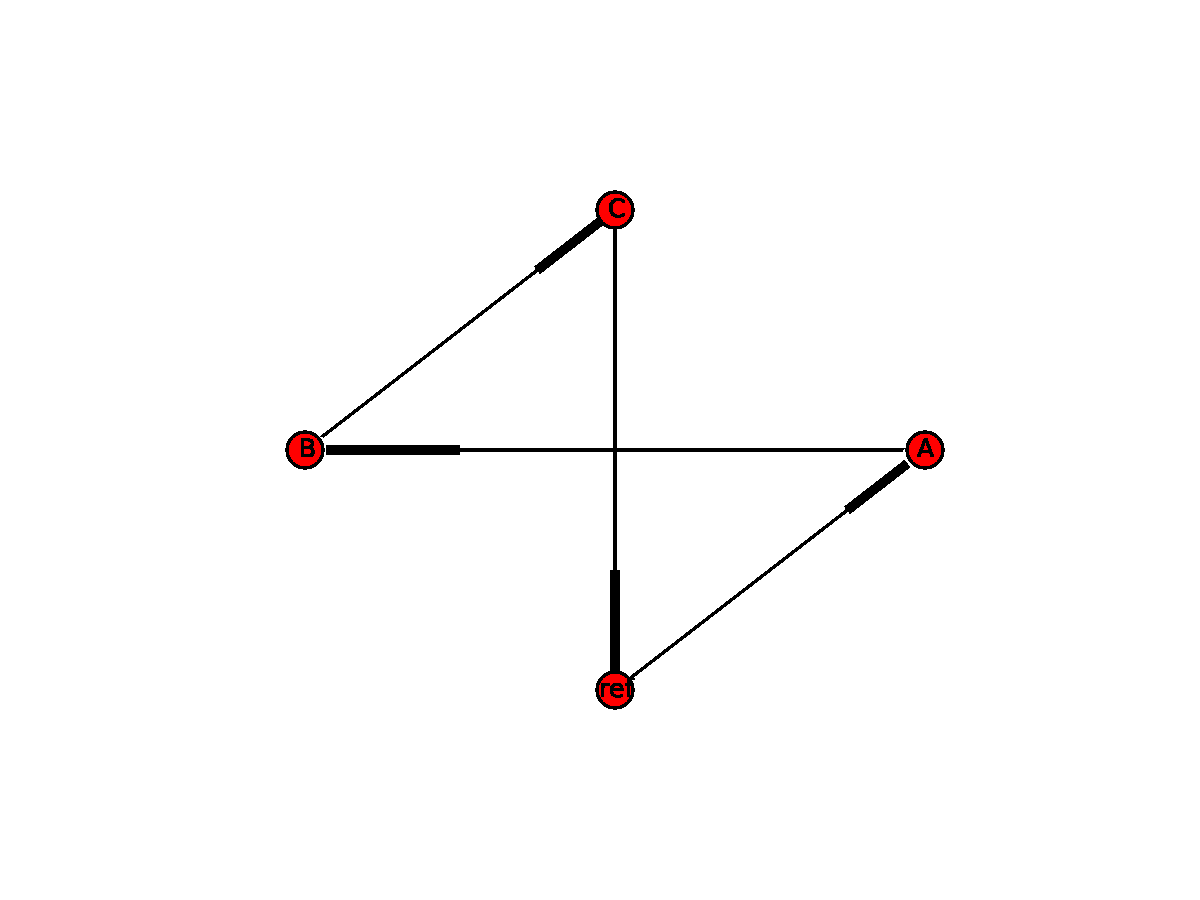
\includegraphics[width=\linewidth]{/Users/afalaize/Developement/repos/pyphs_website/posts/tutos/rlc_graph.pdf}
%
\caption{\label{fig:graph} System's graph with the storage edges in blue, the dissipation edges in green, and the ports edges in red.}
%
\end{center}
%
\end{figure}

% ------------------------------------------------------------------------------
%
\section{Port-Hamiltonian System (\texttt{Core} object)}
%
The Port-Hamiltonian structure in PyPHS is
%
\par\Resize{
$
\left(
  \begin{array}{c}
    \frac{\mathrm d\, \mathbf x}{\mathrm d t} \\
    \mathbf w \\
    \mathbf y \\
    \mathbf {cy} \\
  \end{array}
\right)
=
\left(
  \begin{array}{rrrr}
    \mathbf{M_{xx}} & \mathbf{M_{xw}} & \mathbf{M_{xy}} & \mathbf{M_{xcy}} \\
    \mathbf{M_{wx}} & \mathbf{M_{ww}} & \mathbf{M_{wy}} & \mathbf{M_{wcy}}  \\
    \mathbf{M_{yx}} & \mathbf{M_{yw}} &  \mathbf{M_{yy}} & \mathbf{M_{ycy}}  \\
    \mathbf{M_{cyx}} & \mathbf{M_{cyw}} &  \mathbf{M_{cyy}} & \mathbf{M_{cycy}}  \\
  \end{array}
\right)
\cdot
\left(
  \begin{array}{c}
    \nabla \mathrm H(\mathbf x)\\
    \mathbf z(\mathbf w) \\
    \mathbf u \\
    \mathbf {cu} \\
  \end{array}
\right)
$
}
%
with
%
\par
\Resize{
  $
    \underbrace{
      \left(
      \begin{array}{rrrr}
        \mathbf{M_{xx}} & \mathbf{M_{xw}} & \mathbf{M_{xy}} & \mathbf{M_{xcy}} \\
        \mathbf{M_{wx}} & \mathbf{M_{ww}} & \mathbf{M_{wy}} & \mathbf{M_{wcy}}  \\
        \mathbf{M_{yx}} & \mathbf{M_{yw}} &  \mathbf{M_{yy}} & \mathbf{M_{ycy}}  \\
        \mathbf{M_{cyx}} & \mathbf{M_{cyw}} &  \mathbf{M_{cyy}} & \mathbf{M_{cycy}}  \\
      \end{array}
      \right)
    }_{\mathbf M}
    =
    \underbrace{\left(
      \begin{array}{rrrr}
        \mathbf{J_{xx}} & \mathbf{J_{xw}} & \mathbf{ J_{xy}} & \mathbf{ J_{xcy}} \\
        -^\intercal\mathbf{J_{xw}} & \mathbf{J_{ww}} & \mathbf{J_{wy}} & \mathbf{J_{wcy}}  \\
        -^\intercal\mathbf{J_{xy}} & -^\intercal\mathbf{J_{wy}} &  \mathbf{J_{yy}} & \mathbf{J_{ycy}}  \\
        -^\intercal\mathbf{J_{xcy}} & -^\intercal\mathbf{J_{wcy}} &  -^\intercal\mathbf{J_{ycy}} & \mathbf{J_{cycy}}  \\
      \end{array}
    \right)}_{\mathbf J}
    -
    \underbrace{
      \left(
      \begin{array}{rrrr}
        \mathbf{R_{xx}} & \mathbf{R_{xw}} & \mathbf{ R_{xy}} & \mathbf{ R_{xcy}} \\
        \intercal\mathbf{R_{xw}} & \mathbf{R_{ww}} & \mathbf{R_{wy}} & \mathbf{R_{wcy}}  \\
        ^\intercal\mathbf{R_{xy}} & ^\intercal\mathbf{R_{wy}} &  \mathbf{R_{yy}} & \mathbf{R_{ycy}}  \\
        ^\intercal\mathbf{R_{xcy}} & ^\intercal\mathbf{R_{wcy}} &  ^\intercal\mathbf{R_{ycy}} & \mathbf{R_{cycy}}  \\
      \end{array}
      \right)
    }_{\mathbf R}
  $
}
%
% ------------------------------------------------------------------------------
%
\subsection{Dimensions}
%
The system's dimensions are given below.
%
Notice that a 0 value in the dimensions of the linear parts
$\bullet_{\mathbf{l}} = \bullet-\bullet_{\mathbf{nl}}$ occurs if the system has
not been split.
%
\par  $\dim(\mathbf{l})=$ $ n_\mathbf{l} = 0$\par  $\dim(\mathbf{n_{l}})=$ $ n_\mathbf{n_{l}} = 3$\par  $\dim(\mathbf{x})=$ $ n_\mathbf{x} = 2$\par  $\dim(\mathbf{x_{l}})=$ $ n_\mathbf{x_{l}} = 0$\par  $\dim(\mathbf{x_{nl}})=$ $ n_\mathbf{x_{nl}} = 2$\par  $\dim(\mathbf{w})=$ $ n_\mathbf{w} = 1$\par  $\dim(\mathbf{w_{l}})=$ $ n_\mathbf{w_{l}} = 0$\par  $\dim(\mathbf{w_{nl}})=$ $ n_\mathbf{w_{nl}} = 1$\par  $\dim(\mathbf{y})=$ $ n_\mathbf{y} = 1$\par  $\dim(\mathbf{p})=$ $ n_\mathbf{p} = 0$\par  $\dim(\mathbf{o})=$ $ n_\mathbf{o} = 0$\par  $\dim(\mathbf{cy})=$ $ n_\mathbf{cy} = 0$
%
%
% ------------------------------------------------------------------------------
%
\subsection{Constants}
%
The system's constant substition values are given below.
%
\begin{center}
%
\begin{tabular}{ll}
%
\hline
parameter & value (SI)
\\ \hline
$R_{\mathrm{1}}$ & 1000.0
\\
$L_{\mathrm{1}}$ & 0.05
\\
$C_{\mathrm{1}}$ & 2e-06
\\
\hline
\end{tabular}
%
\end{center}
%
%
% ------------------------------------------------------------------------------
%
\subsection{Internal variables}
%
The system's internal variables are given below.
%
\begin{itemize}
%
\item The \emph{state} $\mathbf x: t\mapsto \mathbf x(t)\in \mathbb R ^{2}$ associated with the system's energy storage:
%
\par\Resize{$ \mathbf{x} = \left(\begin{array}{c}x_{\mathrm{L1}}\\x_{\mathrm{C1}}\end{array}\right)$.}
%
\item The \emph{state increment} $\mathbf{d_x}: t\mapsto \mathbf{d_x}(t)\in \mathbb R ^{2}$ that represents the numerical increment during a single simulation time-step:
%
\par\Resize{$ \mathbf{d_x} = \left(\begin{array}{c}d_{\mathrm{xL1}}\\d_{\mathrm{xC1}}\end{array}\right)$.}
%
\item The \emph{dissipation variable} $\mathbf w: t\mapsto \mathbf w(t)\in \mathbb R^{1}$ associated with the system's energy dissipation:
%
\par\Resize{$ \mathbf{w} = \left(\begin{array}{c}w_{\mathrm{R1}}\end{array}\right)$.}
%
\end{itemize}
%
% ------------------------------------------------------------------------------
%
\subsection{External variables}
%
The controlled system's variables are given below.:
%
\begin{itemize}
%
\item the \emph{input variable} $\mathbf u: t\mapsto \mathbf u(t)\in \mathbb R^{1}$ associated with the system's energy supply (sources):
%
\par\Resize{$ \mathbf{u} = \left(\begin{array}{c}u_{\mathrm{out}}\end{array}\right)$.}
%
\item the \emph{parameters} $\mathbf p: t\mapsto \mathbf p(t)\in \mathbb R^{0}$ associated with variable system parameters:
%
\par\Resize{$ \mathbf p = \mathrm{Empty}$.}
%
\end{itemize}
%
% ------------------------------------------------------------------------------
%
\subsection{Output variables}
%
The output (\textit{i.e.} observed quantities) are:
%
\begin{itemize}
%
\item The \emph{output variable} ${\mathbf y: t\mapsto \mathbf y(t)\in \mathbb R^{1}}$ associated with the system's energy supply (sources):
%
\par\Resize{$ \mathbf y = \left(\begin{array}{c}y_{\mathrm{out}}\end{array}\right)$.}
%
\par\Resize{$ y_{\mathrm{out}} = \frac{1.0}{L_{\mathrm{1}}} \cdot x_{\mathrm{L1}}$.}

%

%
\item The \emph{observer} ${\mathbf o: t\mapsto \mathbf o(t)\in \mathbb R^{0}}$ associated with functions of the above quantities:
%
\par\Resize{$ \mathbf o = \mathrm{Empty}$.}
%

%
\end{itemize}
%
% ------------------------------------------------------------------------------
%
\subsection{Connectors}
%
The inputs and ouputs intended to be connected are given below.
%
\begin{itemize}
%
\item The \emph{connected inputs} ${\mathbf u_c: t\mapsto \mathbf u_c(t)\in \mathbb R^{0}}$
%
\par\Resize{$ \mathbf u_c = \mathrm{Empty}$.}
%
\item The \emph{connected outputs} ${\mathbf y_c: t\mapsto \mathbf y_c(t)\in \mathbb R^{0}}$
%
\par\Resize{$ \mathbf y_c = \mathrm{Empty}$.}
%
\end{itemize}
%

%
% ------------------------------------------------------------------------------
%
\subsection{Constitutive relations}
%
% ------------------------------------------------------------------------------
%
\subsubsection{Storage}
%
The system's \emph{storage function} (Hamiltonian) is:
%
\par\Resize{$ \mathrm H(\mathbf{x}) = \frac{0.5}{L_{\mathrm{1}}} \cdot x_{\mathrm{L1}}^{2} + \frac{0.5}{C_{\mathrm{1}}} \cdot x_{\mathrm{C1}}^{2}$}
%
\par
The gradient of the system's storage function is:
%
\par\Resize{$ \nabla\mathrm H(\mathbf{x}) = \left(\begin{array}{c}g_{\mathrm{xL1}}\\g_{\mathrm{xC1}}\end{array}\right)$}
%
\par\Resize{$ g_{\mathrm{xL1}} = \frac{1.0}{L_{\mathrm{1}}} \cdot x_{\mathrm{L1}}$.}

%
\par\Resize{$ g_{\mathrm{xC1}} = \frac{1.0}{C_{\mathrm{1}}} \cdot x_{\mathrm{C1}}$.}

%

%
\par
The Hessian matrix of the storage function is:
%
\par\Resize{$ \triangle\mathrm H(\mathbf x) = \left(\begin{array}{cc}\frac{1.0}{L_{\mathrm{1}}} & 0\\0 & \frac{1.0}{C_{\mathrm{1}}}\end{array}\right)$}
%
\par
The Hessian matrix of the linear part of the storage function is:
%
\par\Resize{$ \mathbf{Q} = \mathrm{Empty}$}
%
% ------------------------------------------------------------------------------
%
\subsubsection{Dissipation}
%
The dissipation function is:
%
\par\Resize{$ \mathbf z(\mathbf{w}) = \left(\begin{array}{c}z_{\mathrm{R1}}\end{array}\right)$}
%
\par\Resize{$ z_{\mathrm{R1}} = R_{\mathrm{1}} \cdot w_{\mathrm{R1}}$.}

%

%
\par
The jacobian matrix of the dissipation function is:
%
\par\Resize{$ \mathcal J_{\mathbf z}(\mathbf w) = \left(\begin{array}{c}R_{\mathrm{1}}\end{array}\right)$}
%
\par
The jacobian matrix of the linear part of the dissipation function is:
%
\par\Resize{$ \mathbf{Z_l} = \mathrm{Empty}$}
%
% ------------------------------------------------------------------------------
%
\subsection{Structure}
%
The interconnection matrices $\mathbf M=\mathbf J-\mathbf R$ are given below.
%
\subsubsection{$\mathbf M$ structure}
%
\par\Resize{$ \mathbf{M} = \left(\begin{array}{cccc}0 & -1.0 & -1.0 & -1.0\\1.0 & 0 & 0 & 0\\1.0 & 0 & 0 & 0\\1.0 & 0 & 0 & 0\end{array}\right)$}
%
\par\Resize{$ \mathbf{M_{xx}} = \left(\begin{array}{cc}0 & -1.0\\1.0 & 0\end{array}\right)$}
%
\par\Resize{$ \mathbf{M_{xw}} = \left(\begin{array}{c}-1.0\\0\end{array}\right)$}
%
\par\Resize{$ \mathbf{M_{xy}} = \left(\begin{array}{c}-1.0\\0\end{array}\right)$}
%
\par\Resize{$ \mathbf{M_{xcy}} = \mathrm{Empty}$}
%
\par\Resize{$ \mathbf{M_{wx}} = \left(\begin{array}{cc}1.0 & 0\end{array}\right)$}
%
\par\Resize{$ \mathbf{M_{ww}} = \mathrm{Zeros}$}
%
\par\Resize{$ \mathbf{M_{wy}} = \mathrm{Zeros}$}
%
\par\Resize{$ \mathbf{M_{wcy}} = \mathrm{Empty}$}
%
\par\Resize{$ \mathbf{M_{yx}} = \left(\begin{array}{cc}1.0 & 0\end{array}\right)$}
%
\par\Resize{$ \mathbf{M_{yw}} = \mathrm{Zeros}$}
%
\par\Resize{$ \mathbf{M_{yy}} = \mathrm{Zeros}$}
%
\par\Resize{$ \mathbf{M_{ycy}} = \mathrm{Empty}$}
%
\par\Resize{$ \mathbf{M_{cyx}} = \mathrm{Empty}$}
%
\par\Resize{$ \mathbf{M_{cyw}} = \mathrm{Empty}$}
%
\par\Resize{$ \mathbf{M_{cyy}} = \mathrm{Empty}$}
%
\par\Resize{$ \mathbf{M_{cycy}} = \mathrm{Empty}$}
%

%
\subsubsection{$\mathbf J$ structure}
%
\par\Resize{$ \mathbf{J} = \left(\begin{array}{cccc}0 & -1.0 & -1.0 & -1.0\\1.0 & 0 & 0 & 0\\1.0 & 0 & 0 & 0\\1.0 & 0 & 0 & 0\end{array}\right)$}
%
\par\Resize{$ \mathbf{J_{xx}} = \left(\begin{array}{cc}0 & -1.0\\1.0 & 0\end{array}\right)$}
%
\par\Resize{$ \mathbf{J_{xw}} = \left(\begin{array}{c}-1.0\\0\end{array}\right)$}
%
\par\Resize{$ \mathbf{J_{xy}} = \left(\begin{array}{c}-1.0\\0\end{array}\right)$}
%
\par\Resize{$ \mathbf{J_{xcy}} = \mathrm{Empty}$}
%
\par\Resize{$ \mathbf{J_{wx}} = \left(\begin{array}{cc}1.0 & 0\end{array}\right)$}
%
\par\Resize{$ \mathbf{J_{ww}} = \mathrm{Zeros}$}
%
\par\Resize{$ \mathbf{J_{wy}} = \mathrm{Zeros}$}
%
\par\Resize{$ \mathbf{J_{wcy}} = \mathrm{Empty}$}
%
\par\Resize{$ \mathbf{J_{yx}} = \left(\begin{array}{cc}1.0 & 0\end{array}\right)$}
%
\par\Resize{$ \mathbf{J_{yw}} = \mathrm{Zeros}$}
%
\par\Resize{$ \mathbf{J_{yy}} = \mathrm{Zeros}$}
%
\par\Resize{$ \mathbf{J_{ycy}} = \mathrm{Empty}$}
%
\par\Resize{$ \mathbf{J_{cyx}} = \mathrm{Empty}$}
%
\par\Resize{$ \mathbf{J_{cyw}} = \mathrm{Empty}$}
%
\par\Resize{$ \mathbf{J_{cyy}} = \mathrm{Empty}$}
%
\par\Resize{$ \mathbf{J_{cycy}} = \mathrm{Empty}$}
%

%
\subsubsection{$\mathbf R$ structure}
\par\Resize{$ \mathbf{R} = \mathrm{Zeros}$}
%
\par\Resize{$ \mathbf{R_{xx}} = \mathrm{Zeros}$}
%
\par\Resize{$ \mathbf{R_{xw}} = \mathrm{Zeros}$}
%
\par\Resize{$ \mathbf{R_{xy}} = \mathrm{Zeros}$}
%
\par\Resize{$ \mathbf{R_{xcy}} = \mathrm{Empty}$}
%
\par\Resize{$ \mathbf{R_{wx}} = \mathrm{Zeros}$}
%
\par\Resize{$ \mathbf{R_{ww}} = \mathrm{Zeros}$}
%
\par\Resize{$ \mathbf{R_{wy}} = \mathrm{Zeros}$}
%
\par\Resize{$ \mathbf{R_{wcy}} = \mathrm{Empty}$}
%
\par\Resize{$ \mathbf{R_{yx}} = \mathrm{Zeros}$}
%
\par\Resize{$ \mathbf{R_{yw}} = \mathrm{Zeros}$}
%
\par\Resize{$ \mathbf{R_{yy}} = \mathrm{Zeros}$}
%
\par\Resize{$ \mathbf{R_{ycy}} = \mathrm{Empty}$}
%
\par\Resize{$ \mathbf{R_{cyx}} = \mathrm{Empty}$}
%
\par\Resize{$ \mathbf{R_{cyw}} = \mathrm{Empty}$}
%
\par\Resize{$ \mathbf{R_{cyy}} = \mathrm{Empty}$}
%
\par\Resize{$ \mathbf{R_{cycy}} = \mathrm{Empty}$}
%

%

%
% -----------------------------------------------------------------------------
%
% -----------------------------------------------------------------------------
%
\end{document}
